\documentclass[10pt]{article}
%\usepackage{mathpazo}
%\usepackage{euler}
\usepackage[utf8]{inputenc}
\usepackage{amsmath}
\usepackage{amsfonts}
\usepackage{amssymb}
\usepackage{amsthm}
\usepackage{graphicx}
\usepackage{enumerate}
\usepackage{ragged2e}
\usepackage{xcolor}
\usepackage[spanish,onelanguage]{algorithm2e}
%\setlength{\parindent}{0em}
\usepackage[left=2.9cm,right=2.9cm,top=2cm,bottom=2.5cm]{geometry}
\usepackage{pgfplots,tikz,tikz-cd}
\pgfplotsset{compat=1.17}
\author{Ángel Ríos San Nicolás}
\theoremstyle{definition}
\newtheorem{ejer}{Ejercicio}
\newtheorem*{sol}{Solución}
\title{Geometría Discreta y Computación}
\date{Hoja 2--$h$-vectores, politopos regulares\\ 18 de enero de 2020}
\newcommand{\R}{\mathbb{R}}
\begin{document}

\maketitle
\begin{ejer}$4$\textbf{-politopos regulares.} Para cada uno de los cinco $3$-politopos regulares, considera las siguientes longitudes: su lado $l$, su radio $r$ (distancia de un vértice al centro) y su diagonal $d$ (distancia $AC$ donde $ABC$ son vértices consecutivos de una faceta; si la faceta es un triángulo, $d=l$).
Llamamos ``apertura central'' de $P$ al cociente $l/r$ y ``apertura facial'' a $d/l$. 
\begin{enumerate}[(a)]
\item Justifica la siguiente afirmación: ``Existe un $4$-politopo regular con faceta $P$ y figura de vértice $Q$ si, y solo si, la apertura central de $Q$ es estrictamente mayor que la apertura facial de $P$.'' 

\item Usando ese criterio, demuestra que solo seis de las 11 posibilidades de $(p,q,r)$ producen $4$-politopos regulares.%
%\footnote{En algunos casos no necesitas calcular las aperturas exactamente, solo usar desigualdades entre ellas; pero la apertura central del icosaedro y la apertura facial del dodecaedro son fáciles de calcular recordando que la razón entre la diagonal y el lado de un pentágono regular es la razón aúrea $\phi=\frac{1+\sqrt5}2$}
\end{enumerate}
\end{ejer}
\begin{sol}\leavevmode
\begin{enumerate}[(a)]
\item Si partimos de la figura de vértice $Q$ y trazamos segmentos desde el centro hasta los vértices, la razón del lado y su longitud mide la apertura central de $Q$. Para poder colocar una copia de la faceta $P$ en el interior de $Q$ de manera que no toque ni corte estos segmentos es una condición necesaria y suficiente que la apertura facial de $P$ sea estrictamente menor porque entonces, independientemente del lado, el ángulo sólido de una faceta de $Q$ será más grande y colocando $P$ sobra espacio en $\mathbb{R}^3$. Colocando más facetas, el espacio que sobra permite moverse en la cuarta dimensión de manera que la construcción se cierra en $\mathbb{R}^4$ en un $4$-politopo regular con faceta $P$ y figura de vértice $Q$, análogamente a la construcción de los $3$-politopos regulares a partir de polígonos regulares. Debe cerrarse bien porque de lo contrario tendríamos un recubrimiento no trivial de la esfera $\mathbb{S}^3$, que es una contradicción con el hecho de que sea simplemente conexa.
\item Calculamos las aperturas central y facial de cada $3$-politopo regular. Como el radio y la diagonal serán múltiplos del lado, podemos suponer un lado conveniente para calcular los cocientes.
\begin{itemize}
    \item Tetraedro (3,3)
    
    Se puede realizar el tetraedro como la envolvente convexa de los puntos \[\left\{\left(\pm 1,0,-\frac{1}{\sqrt{2}}\right),\left(0,\pm 1,\frac{1}{\sqrt{2}}\right)\right\}\] con lo que tenemos que la longitud y la diagonal son $l=2=d$ y el centro es $(0,0,0)$ así que el radio es $r=\left(1+\left(-\frac{1}{\sqrt{2}}\right)^2\right)^\frac{1}{2}=\frac{\sqrt{3}}{\sqrt{2}}=\frac{\sqrt{6}}{2}$.
    
    Apertura central: $\frac{l}{r}=\frac{2}{3}\sqrt{6}$.
    Apertura facial: $\frac{d}{l}=1$.
    
    \item Cubo (4,3)
    
    Se puede realizar el cubo como la envolvente convexa de los puntos \[\{(0,0,0),(1,0,0),(0,1,0),(0,0,1),(1,1,0),(1,0,1),(0,1,1),(1,1,1)\}\]
    con lo que tenemos que el lado es $l=1$, la diagonal es $\sqrt{2}$ y el centro es $\left(\frac{1}{2},\frac{1}{2},\frac{1}{2}\right)$ así que el radio es $r=\frac{\sqrt{3}}{2}.$
    
    Apertura central: $\frac{l}{r}=\frac{2}{3}\sqrt{3}.$
    Apertura facial: $\frac{d}{l}=\sqrt{2}$.
    \item Octaedro (3,4)
    
    Se puede realizar el octaedro como la envolvente convexa de los puntos 
    \[\{(1,0,0),(-1,0,0),(0,1,0),(0,-1,0),(0,0,1),(0,0,-1)\}\]
    con lo que tenemos que el lado y la diagonal son $l=\sqrt{2}=d$ y el centro es $(0,0,0)$ así que el radio es $1$, la mitad de la diagonal del cuadrado de lado $\sqrt{2}$.
    
    Apertura central: $\frac{l}{r}=\sqrt{2}$.
    Apertura facial: $\frac{d}{l}=1$
    
    
    \item Dodecaedro (5,3)
    
    Se puede realizar el dodecaedro como la envolvente convexa de los puntos \[\left\{\left(\pm 1,\pm 1,\pm 1\right),\left(0,\pm\varphi,\pm\frac{1}{\varphi}\right),\left(\pm\frac{1}{\varphi}, 0,\pm\varphi\right),\left(\pm \varphi,\pm\frac{1}{\varphi},0\right)\right\}\]
    con lo que tenemos que el lado es $l=\frac{2}{\varphi}$, la diagonal es $d=\frac{2}{\varphi}\varphi=2$ y el centro es $(0,0,0)$ así que el radio es $r=\left(1^2+1^2+1^2\right)^{\frac{1}{2}}=\sqrt{3}$
    
    Apertura central: $\frac{l}{r}=\frac{2}{3\varphi}\sqrt{3}$.
    Apertura facial: $\frac{d}{l}=\varphi$.
    
    \item Icosaedro (3,5)
    
    Se puede realizar el icosaedro como la envolvente convexa de los puntos \[\left\{\left(0,1,\pm\varphi\right),\left(\pm\varphi,0,\pm 1\right),\left(\pm\ 1,\pm\varphi,0\right)\right\}\]
    con lo que tenemos que el lado y la diagonal son $l=2=d$ y el centro es $(0,0,0)$ así que el radio es $r=\left(1+\varphi^2\right)^\frac{1}{2}=\sqrt{\varphi+2}$.
    
    Apertura central: $\frac{l}{r}=\frac{2}{\sqrt{\varphi+2}}$.
    Apertura facial: $\frac{d}{l}=1$.
\end{itemize}
La existencia o no del $4$-politopo regular correspondiente a cada una de las $11$ posibilidades del símbolo de Schläfli viene recogida en la siguiente tabla. La desigualdad $d/l<l/r$ compara, por el criterio anterior, si la apertura facial de la faceta es estrictamente menor que la apertura central de la figura de vértice.
\begin{center}
\begin{tabular}{|c|c|c|c|c|}
\hline Símbolo de Schläfli    & Faceta     & Figura de vértice & $4$-politopo regular  & $d/l < l/r$ \\
\hline $(3,3,3)$              & Tetraedro  & Tetraedro         & $4$-símplice          & $1<2\sqrt{6}/3$\\
\hline $(3,3,4)$              & Tetraedro  & Octaedro          & \textit{cross-politopo} & $1<\sqrt{2}$\\
\hline $(3,3,5)$              & Tetraedro  & Icosaedro         & $600$-celda           & $1<2/\sqrt{\varphi+2}$\\
\hline $(4,3,3)$              & Cubo       & Tetraedro         & $4$-cubo              & $\sqrt{2}<2\sqrt{6}/3$\\
\hline $(4,3,4)$              & Cubo       & Octaedro          & $\nexists$            & $\sqrt{2}\not<\sqrt{2}$\\
\hline $(4,3,5)$              & Cubo       & Icosaedro         & $\nexists$            & $\sqrt{2}\not< 2/\sqrt{\varphi+2}$\\
\hline $(3,4,3)$              & Octaedro   & Cubo              & $24$-celda            & $1<2\sqrt{3}/3$\\
\hline $(5,3,3)$              & Dodecaedro & Tetraedro         & $120$-celda           & $\varphi<2\sqrt{6}/3$\\
\hline $(5,3,4)$              & Dodecaedro & Octaedro          & $\nexists$            & $\varphi\not<\sqrt{2}$\\
\hline $(5,3,5)$              & Dodecaedro & Icosaedro         & $\nexists$            & $\varphi\not< 2/\sqrt{\varphi+2}$\\
\hline $(3,5,3)$              & Icosaedro  & Dodecaedro        & $\nexists$            & $1\not < 2\sqrt{3}/(3\varphi)$\\ \hline
\end{tabular}\end{center}
\end{enumerate}
\end{sol}

\begin{ejer}\textbf{El }$d$\textbf{-cubo.} Sea $C_d=[-1,1]^d$ el cubo regular de dimensión $d$ centrado en el origen. 
\begin{enumerate}[(a)]
\item Calcula el $f$-vector de $C_d$ de dos maneras: 
\begin{enumerate}[i.]
\item Usando la descomposición $C_d= C_{d-1}\times \{-1\} \quad\dot\cup\quad C_{d-1}\times (0,1) \quad\dot\cup\quad C_{d-1}\times \{1\}$.
\item Encontrando una biyección entre las caras de dimensión $k$ y los vectores de $\{-1,0,1\}^d$ con $k$ ceros.
\end{enumerate}

\item Demuestra que el número de banderas de $C_d$ es $d!\times 2^d$, que coincide con el orden de su grupo de simetrías (permutaciones y/o cambios de signo de coordenadas).

\item Calcula el $h$-vector del polar de $C_d$, el llamado \emph{cross-politopo} de dimensión $d$.
\end{enumerate}
{\bf Nota:} $C_d$ y su polar son politopos regulares con símbolo de Schl\"afli $(4,3,\dots,3)$ y $(3,\dots,3,4)$. Junto con el $d$-símplice son los únicos $d$-politopos regulares para $d\ge 5$.


\end{ejer}
\begin{sol}\leavevmode
\begin{enumerate}[(a)]
\item
\begin{enumerate}[i.]
\item Denotamos mediante $f_i^d$ al número de caras de dimensión $i$ de $C_d$, el cubo regular de dimensión $d$ y $f^d$ al $f$-vector completo de $C_d$. Esto es un abuso de notación respecto a la exponenciación, pero no habrá ambigüedad. Sabemos que $f_{-1}^d=1=f_d^d$ para todo $d\in\mathbb{N}$, $d\geq 1$. Nos centramos en el resto de componentes. Afirmamos que para todos $d,i\in\mathbb{N}$, $d\geq 1$, $0\leq i\leq d-1$, se cumple
\[f_i^d=2^{d-i}\begin{pmatrix}d\\i\end{pmatrix}\]
y lo probamos para cada $i$ por inducción en la dimensión $d$. Utilizando la descomposición, vamos a ver que podemos poner $f_i^d$ en función de $f_i^{d-1}$ y $f_{i-1}^{d-1}$.
% En dimensión $1$, es $C_{1}=[-1,1]$ que tiene $2$ vértices con lo que $f^1=(1,2,1)$.

% En dimensión $2$, es $C_{2}=[-1,1]^2$ que tiene $4$ vértices y $4$ aristas con lo que $f^2=(1,4,4,1)$.

% En dimensión $3$, es $C_{3}=[-1,1]^3$ que tiene $8$ vértices, $12$ aristas y $6$ caras con lo que $f^3=(1,8,12,6,1)$.

% En dimensión $4$, es $C_{4}=[-1,1]^4$ que tiene $16$ vértices, $32$ aristas, $24$ caras y $8$ facetas con lo que $f^4=(1,16,32,24,8,1)$.
Sabemos que dado $C_{d-1}$, la construcción de $C_d$ es cilíndrica, contiene dos copias de $C_{d-1}$ unidas por caras de dimensión menor. Al multiplicar por $(-1,1)$, cada punto genera una arista, cada arista una cara de dimensión $2$, cada cara de dimensión $2$ una cara de dimensión $3$... En general, cada cara de dimensión $k$, genera una cara de dimensión $k+1$. Por lo tanto, se cumple \[f_i^d=2f_i^{d-1}+f_{i-1}^{d-1}\text{ para todo $i\in\{0,\ldots,d-1\}$}.\]
El sumando $2f_i^{d-1}$ por las dos copias de $C_{d-1}$ y el sumando $f_{i-1}^{d-1}$ porque hay que añadir tantas caras de dimensión $i$ como caras de dimensión $i-1$ del cubo de dimensión $C_{d-1}$.
En dimensión $1$, se cumple $2=2^{1-0}\begin{pmatrix}1\\ 0\end{pmatrix}$. Suponemos que se cumple para $d-1$, es decir, que
\[f_i^{d-1}=2^{d-1-i}\begin{pmatrix}d-1\\ i\end{pmatrix} \text{ para todo $i\in\{0,\ldots,d-1\}$}.\]
Aplicando las fórmulas anteriores,
\[f_i^d=2\cdot 2^{d-1-i}\begin{pmatrix}d-1\\ i\end{pmatrix}+2^{d-1-i+1}\begin{pmatrix}d-1\\ i-1\end{pmatrix}=2^{d-i}\left(\begin{pmatrix}d-1\\i\end{pmatrix}+\begin{pmatrix}d-1\\i-1\end{pmatrix}\right)=2^{d-i}\begin{pmatrix}d\\i\end{pmatrix}\]
como queríamos probar.
\item
Buscamos ahora una biyección entre el número de caras de $C_d$ de dimensión $k$ y el número de vectores de $\{-1,0,1\}^d$ con $k$ ceros que tiene $2^{d-k}\begin{pmatrix}d\\ k\end{pmatrix}$ elementos porque se corresponde a escoger las $k$ coordenadas de ceros y, para cada elección, dar valor $-1$ o $1$ al resto de coordenadas.

Observamos que $C_d$ está realizado como $d$-cubo unitario centrado en el origen.

En dimensión $1$, los vértices son $-1$ y $1$ con lo que $f_0^2=2$ es el número de vectores de $\{-1,1\}$ El punto medio de la arista es $0$ y $f_1^1=1$ es el número de vectores de $\{0\}$.

En dimensión $2$, es el cuadrado de vértices $(\pm 1,\pm 1)$ con las cuatro elecciones posibles de signos. Observamos que los puntos medios de las aristas son los elementos de $\{0,1\}^2$ y $\{-1,0\}^2$ y tenemos que $f_0^2=4$ es el número de vectores sin ceros $(\pm 1,\pm 1)$ y $f_1^2=4$ es el número $|\{-1,0\}^2\cup\{0,1\}^2|$ de vectores con un cero.

Esto se puede generalizar en cualquier dimensión $d$. Por la construcción de $C_d$. Dado $v\in\{-1,0,1\}^d$ con $k$ ceros, podemos considerar los $2^k$ elementos obtenidos sustituyendo los ceros por $-1$ o $1$. Claramente son vértices de $C_d$ y, por ser $2^k$ con $d-k$ coordenadas iguales, definen una única cara de $C_d$ de dimensión $k$ al tomar su envolvente convexa, que contiene a $v$ porque se puede poner como la combinación convexa $v=\frac{1}{2}v_{-1}+\frac{1}{2}v_{1}$ siendo $v_{-1}$ y $v_{1}$ los vectores obtenidos al sustituir los ceros todos por $-1$ y todos por $1$ respectivamente. Se puede ver así $v$ como el centro de la cara. La existencia y unicidad define una biyección entre las caras de $C_d$ de dimensión $k$ y los elementos de $C_d$ con $k$ ceros.
\end{enumerate}
\item Probamos que el número de banderas de $C_d$ es $d!2^d$ por inducción en la dimensión $d$. Si $d=1$, el número de banderas es $2=1!2^1$ porque tenemos dos vértices. Suponemos que se cumple para $d-1$, es decir, que el número de banderas de $C_{d-1}$ es $(d-1)!2^{d-1}$. Recordamos ahora la descomposición \[C_d=\left(C_{d-1}\times\{-1\}\right)\dot\bigcup \left(C_{d-1}\times (-1,1)\right)\dot\bigcup\left( C_{d-1}\times\{1\}\right)=C_{d-1}\times [-1,1]\]
de la que se deduce que las facetas de $C_d$ son copias de $C_{d-1}$. Por lo tanto, para construir una bandera de $C_d$ solo hay que escoger una faceta, de las que hay
\[f_{d-1}^d=2^{d-(d-1)}\begin{pmatrix}d\\ d-1\end{pmatrix}=2\frac{d!}{(d-1)!1!}=2\frac{d(d-1)!}{(d-1)!}=2d\]
opciones. La faceta escogida tiene, por hipótesis de inducción, $(d-1)!2^{d-1}$ banderas. Por lo tanto, el número de banderas de $C_d$ es el producto $2d(d-1)!2^{d-1}=d!2^d$ como queríamos probar.

En $d$ coordenadas, el número de cambios de signo es $2^d$ y el de permutaciones es $d!$, por lo tanto, el número de simetrías de $C_d$ es $d!2^d$, igual que el número de banderas y el $d$-cubo $C_d$ es un $d$-politopo regular.
\item Sabemos que el $f$-vector del \textit{cross-politopo} de dimensión $d$ es el reverso del $f$-vector de $C_d$. Si el $f$-vector del $d$-cubo es $\tilde{f}^d=\left(1,f_0^d,f_1^d,\ldots, f_{d-1}^d,1\right)$, entonces el $f$-vector del \textit{cross-politopo} de dimensión $d$ es $\tilde{f}^d=\left(1,f_{d-1}^d,\ldots,f_2^d,f_1^d,1\right)$ con lo que el coeficiente general es
\[\tilde{f}_i^d=f_{d-(i+1)}^d=2^{d-(d-(i+1))}\begin{pmatrix}d\\ d-(i+1)\end{pmatrix}=2^{i+1}\begin{pmatrix}d\\ i+1\end{pmatrix}.\]
Calculamos el $h$-vector $\tilde{h}^d$ del \textit{cross-politopo} mediante polinomios. El polinomio $\tilde{F}^d$ asociado al $f$-vector $\tilde{f}^d$ es
\[\tilde{F}^d(X)=\sum_{i=0}^d\tilde{f}_{i-1}^dX^{d-i}=\sum_{i=0}^d\begin{pmatrix}d\\ i\end{pmatrix}2^iX^{d-i}=(2+X)^d.\]
Por lo tanto, el polinomio $\tilde{H}^d$ asociado al $h$-vector $\tilde{h}$ está dado por
\[\tilde{H}^d(X)=F(1-X)=(1+X)^d=\sum_{i=0}^d\begin{pmatrix}d\\ i\end{pmatrix}X^{d-i}.\]
El $h$-vector $\tilde{h}^d$ del \textit{cross-politopo} de dimensión $d$ es 
\[\tilde{h}^d_i=\begin{pmatrix}d\\ i\end{pmatrix}.
\]

\end{enumerate}
\end{sol}

\begin{ejer}\textbf{La $24$-celda.} Sea $P$ la envolvente convexa de los siguientes 24 puntos en $\R^4$: los 16 vértices $(\pm 1, \pm 1, \pm 1, \pm 1)$ del $4$-cubo y los 8 vértices $\pm 2 e_i$ de un cross-politopo (dual del cubo) dilatado a tamaño doble. Obsérvese que los 24 vértices quedan en una esfera de radio $2$.
\begin{enumerate}[(a)]
\item P tiene la siguiente descripción por facetas, con $24$ desigualdades (son $24$ porque hay seis maneras de elegir $i$ y $j$, y para cada una hay cuatro elecciones de signos):%
%\footnote{Se trata de ver que las 24 desigualdades son válidas en los 24 puntos, pero también que no nos faltan facetas. Para esto último, elige una faceta $F$ (son todas equivalentes por permutación y/o cambio de signo de las coordenadas) y observa que  tanto su descripción por vértices (envolvente convexa de los vértices que quedan en $F$) como su descripción por facetas (desigualdades de $P$ que pasan por al menos tres vértices de $F$) producen el mismo $3$-politopo, un octaedro. Como la descripción por facetas es completa restringida a $F$ (y a todas las demás facetas),  es completa globalmente. Puedes considerar el siguiente cambio de variables, que es ortogonal y manda la faceta $x_1+x_2=2$ al hiperplano $y_1=1$:
%\[
%y_1 = \frac{x_1+x_2}2,\quad
%y_2 = \frac{x_1-x_2}2,\quad
%y_3 = \frac{x_3+x_4}2,\quad
%y_4 = \frac{x_3-x_4}2.\quad
%\]
%}
\[
P = \left\{(x_1,x_2,x_3,x_4) \in \R^4 : \quad \pm \, x_i \pm x_j \le 2, \quad 1\le i < j \le 4 \right\}.
\]

\item Demuestra que $P$ es regular, es decir que el orden de su grupo de simetrías coincide con el número de banderas.%
%\footnote{Para contar banderas, multiplica el número de facetas por las banderas que usan cada faceta; para el grupo de simetrías, es obvio que contiene al subgrupo de orden $24\times 16$ formado por permutaciones y/o cambio de signo de coordenadas. Encuentra una simetría adicional, de orden tres, que no está en ese subgrupo y que intercambia cíclicamente los vértices $(2,0,0,0)$, $(1,1,1,1)$ y $(1,1,1,-1)$.}

\item Calcula el $f$-vector de $P$, y el $f$-vector $P'$ de un politopo simplicial obtenido ``dividiendo cada octaedro en cuatro tetraedros con una arista común'' (nota: este es el politopo que se obtendría perturbando ligeramente los 24 vértices para que no haya más de cuatro en ningún hiperplano). Como $P'$ es simplicial, calcula su $h$-vector.

\end{enumerate}
\small {\bf Nota:}  $P$ es el $4$-politopo regular con símbolo de Schl\"afli $(3,4,3)$, y es su propio polar (esto último se sigue de que el símbolo de Schl\"afli es simétrico, pero también de que la transformación de coordenadas sugerida en el apartado (a) manda los 24 vértices de $P$ sobre los 24 vectores $\pm e_i \pm e_j$ normales a las facetas).
\end{ejer}
\begin{sol}\leavevmode
\begin{enumerate}[(a)]
    \item Vamos a ver primero que los vértices de la $24$-celda cumplen las desigualdades de $P$.
    Si escogemos un vértice $(\pm 1,\pm 1,\pm 1,\pm 1)$ del cubo con cualquier elección de signos en cada coordenada, tenemos que las diferentes posibilidades son
    \begin{align*}
    1+1 & = 2\\
    1-1 & = 0\\
    -1+1 & = 0\\
    -1-1 & = -2
    \end{align*}
    con lo que se cumplen $\pm x_i\pm x_j\leq 2$ para $1\leq i<j\leq 2$.
    
    Si escogemos un vértice $2e_i$ con $i\in\{1,2,3,4\}$ del \textit{cross-politopo} dual del cubo a tamaño doble, se cumple que una coordenada es $2$ y el resto cero con lo que en las desigualdades de $P$ tenemos que si o $x_i=2$ o $x_j=2$, entonces
    \begin{align*}
    x_i+x_j & = 2\\
    x_i-x_j & = 2\\
    -x_i+x_j & = -2\\
    -x_i-x_j & = -2
    \end{align*}
    y claramente también $\pm x_i\pm x_j\leq 2$ para $1\leq i<j\leq 2$. Si $x_i,x_j\neq 2$, todas las sumas son $0\leq 2$.
    
    Tenemos que ver que no faltan facetas. Escogemos una faceta, por ejemplo, $F: x_1+x_2=2$ y vamos a probar que tanto su decripción por vértices como su descripción por facetas definen el mismo $3$-politopo, un octaedro.
    \begin{itemize}
        \item Descripción de $F$ por vértices.
        Calculamos los vértices de la $24$-celda que cumplen la desigualdad de la faceta $F$. Los vértices cuyas dos primeras coordenadas suman $2$ son 
        \[S=\{(1,1,1,1),(1,1,-1,1),(1,1,1,-1),(1,1,-1,-1),(2,0,0,0),(0,2,0,0)\}\]
        Consideramos el cambio de variable
        \[
        y:\mathbb{R}^4\longrightarrow \mathbb{R}^4,
        (x_1,x_2,x_3,x_4)\longmapsto y(x_1,x_2,x_3,x_4)=\left(\frac{x_1+x_2}{2},\frac{x_1-x_2}{2},\frac{x_3+x_4}{2},\frac{x_3-x_4}{2}\right).\]
        Aplicamos el cambio a los vértices de la faceta y tenemos
        \begin{align*}
            y(1,1,1,1)  & = (1,0,1,0)\\
            y(1,1,-1,1) & = (1,0,0,-1)\\
            y(1,1,1,-1) & = (1,0,0,1)\\
            y(1,1,-1-1) & = (1,0,-1,0)\\
            y(2,0,0,0)  & = (1,1,0,0)\\
            y(0,2,0,0)  & = (1,-1,0,0)
        \end{align*}
        Observamos que, como $y$ transforma la faceta $x_1+x_2=2$ en el hiperplano $y_1=1$, todas los puntos tienen coordenada $1$. Proyectando en ese hiperplano, podemos ver los puntos en $\mathbb{R}^3$ como $\{(\pm1 ,0,0),(0,\pm 1,0),(0,0,\pm 1)\}$ cuya envolvente convexa es claramente un octaedro porque consiste en dos pirámides de base cuadrada unidas por sus bases.
\begin{center}
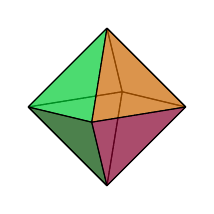
\begin{tikzpicture}[line join=bevel,z=-5.5]
\coordinate (A1) at (0,0,-1);
\coordinate (A2) at (-1,0,0);
\coordinate (A3) at (0,0,1);
\coordinate (A4) at (1,0,0);
\coordinate (B1) at (0,1,0);
\coordinate (C1) at (0,-1,0);

\draw (A1) -- (A2) -- (B1) -- cycle;
\draw (A4) -- (A1) -- (B1) -- cycle;
\draw (A1) -- (A2) -- (C1) -- cycle;
\draw (A4) -- (A1) -- (C1) -- cycle;
\draw [fill opacity=0.7,fill=green!80!blue] (A2) -- (A3) -- (B1) -- cycle;
\draw [fill opacity=0.7,fill=orange!80!black] (A3) -- (A4) -- (B1) -- cycle;
\draw [fill opacity=0.7,fill=green!30!black] (A2) -- (A3) -- (C1) -- cycle;
\draw [fill opacity=0.7,fill=purple!70!black] (A3) -- (A4) -- (C1) -- cycle;
\end{tikzpicture}\end{center}
        
        \item Descripción de $F$ por facetas.
        Tenemos que calcular las desigualdades de $P$ que pasan por al menos tres vértices de la faceta $F$. Los vértices son los elementos del conjunto $S$ que calculamos antes. Los denotamos como sigue
        \begin{align*}
            P_1 & = (1,1,1,1)\\
            P_2 & = (1,1,-1,1)\\
            P_3 & = (1,1,1,-1)\\
            P_4 & = (1,1,-1,-1)\\
            P_5 & = (2,0,0,0)\\
            P_6 & = (0,2,0,0).
        \end{align*}
        y denotamos $\tilde{P}_i=y(P_i)$ para cada $i\in\{1,2,3,4,5,6\}$.
    Con esta notación, comprobamos qué vértices cumplen cada desigualdad de $P$ con igualdad.
    \[\begin{array}{|r|c|}
        \hline \multicolumn{1}{|c|}{\text{Igualdad}} & \text{Vértices}  \\
        \hline x_1+x_2=2 & P_1,P_2,P_3,P_4,P_5,P_6\\
        \hline x_1-x_2=2 & P_5\\
        \hline -x_1+x_2=2 & P_6\\
        \hline -x_1-x_2=2 & \emptyset\\
        
        \hline x_1+x_3=2 & P_1,P_3,P_5\\
        \hline x_1-x_3=2 & P_2,P_4,P_5\\
        \hline -x_1+x_3=2 & \emptyset\\
        \hline -x_1-x_3=2 & \emptyset\\
        
        \hline x_1+x_4=2 & P_1,P_2,P_5\\
        \hline x_1-x_4=2 & P_3,P_4,P_5\\
        \hline -x_1+x_4=2 & \emptyset\\
        \hline -x_1-x_4=2 & \emptyset\\
        
        \hline x_2+x_3=2 & P_1,P_3,P_6\\
        \hline x_2-x_3=2 & P_2,P_4,P_6\\
        \hline -x_2+x_3=2 & \emptyset\\
        \hline -x_2-x_3=2 & \emptyset\\
        
        \hline x_2+x_4=2 & P_1,P_2,P_5\\
        \hline x_2-x_4=2 & P_3,P_4,P_6\\
        \hline -x_2+x_4=2 & \emptyset\\
        \hline -x_2-x_4=2 & \emptyset\\
        
        \hline x_3+x_4=2 & P_1\\
        \hline x_3-x_4=2 & P_3\\
        \hline -x_3+x_4=2 & \emptyset\\
        \hline -x_3-x_4=2 & P_4\\ \hline
    \end{array}\]
    Observamos que los vértices $P_i,P_j,P_k$ con $i,j,k$ distintos dos a dos que verifican una misma desigualdad de $P$ con igualdad se corresponden precisamente con los puntos $\tilde{P}_i,\tilde{P}_j,\tilde{P}_k$ que pertencen a $\mathbb{R}^3$ salvo proyección y que definen una cara del octaedro. La región que encierra el conjunto de ecuaciones con esa propiedad sobre los puntos es precisamente el octaedro.
    \end{itemize}
    \item Para probar que es regular, tenemos que ver que el orden de su grupo de simetrías coincide con el número de banderas. Para contar las banderas, multiplicamos el número de facetas, $24$, por el número de banderas que inciden en cada faceta, pero estas son las banderas del octaedro.
    
    El octaedro tiene $6$ vértices, en cada vértice inciden $4$ aristas y en cada arista inciden $2$ caras. El número de banderas del octaedro es $6\cdot 4\cdot 2=48$. Por lo tanto, el número de banderas de la $24$-celda es $24\cdot 48=1152$.
    El grupo de simetrías de la $24$-celda contiene el subgrupo de orden $24\cdot 16$ de las permutaciones y cambios de coordenadas. Buscamos una simetría $\sigma$ del politopo tal que $\sigma((2,0,0,0))=(1,1,1,1)$, $\sigma((1,1,1,1))=(1,1,1,-1)$ y $\sigma((1,1,1,-1))=(2,0,0,0)$, es decir, $\sigma\left(P_5\right)=P_1$, $\sigma\left(P_1\right)=P_3$ y $\sigma\left(P_3\right)=P_5$ con la notación anterior para los vértices de la faceta $F$. Pero sabemos que estos vértices definen un octaedro que lo podemos ver en $\mathbb{R}^3$ por el cambio de coordenadas $y$. La simetría que buscamos es esencialmente una simetría $\tilde{\sigma}$ del octaedro que cumple $\tilde{\sigma}\left(\tilde{P}_5\right)=\tilde{P}_1$, $\tilde{\sigma}\left(\tilde{P}_1\right)=\tilde{P}_3$ y $\tilde{\sigma}\left(\tilde{P}_3\right)=\tilde{P}_5$. Claramente, deja fijo el centro del octaedro, que es el origen $(0,0,0)$. Calculamos el punto de $\mathbb{R}^4$ que se corresponde con el origen por el cambio de coordenadas y la proyección, es decir, $y^{-1}((1,0,0,0))=(1,1,0,0)$.
    
    La simetría  $\sigma$ está dada respecto de la base $\{P_5,P_1,P_3,(1,1,0,0)\}$ por 
    \[M=\begin{pmatrix}0 & 0 & 1 & 0\\
    1 & 0 & 0 & 0\\
    0 & 1 & 0 & 0\\
    0 & 0 & 0 & 1
    \end{pmatrix}.\]
    Por lo tanto, respecto de la base canónica, tiene como matriz
    \[\sigma = \begin{pmatrix}2 & 1 & 1 & 1\\
    0 & 1 & 1 & 1\\
    0 & 1 & 1 & 0\\
    0 & 1 & -1 & 0\end{pmatrix}\begin{pmatrix}0 & 0 & 1 & 0\\
    1 & 0 & 0 & 0\\
    0 & 1 & 0 & 0\\
    0 & 0 & 0 & 1
    \end{pmatrix}\begin{pmatrix}\frac{1}{2} & \frac{1}{2} & 0 & 0\\
    0 & 0 & \frac{1}{2} & \frac{1}{2}\\
    0 & 0 & \frac{1}{2} & -\frac{1}{2}\\
    0 & 1 & -1 & 0\end{pmatrix}=\frac{1}{2}\begin{pmatrix}1 & 1 & 1 & -1\\
    1 & 1 & -1 & 1\\
    1 & -1 & 1 & 1\\
    1 & -1 & -1 & -1\end{pmatrix}.\]
    Esta aplicación transforma entre sí vértices de la faceta del politopo y por lo tanto también caras entre sí, es decir, es una simetría del octaedro correspondiente: $\sigma(P_2)=P_6$, $\sigma(P_6)=P_4$, $\sigma(P_4)=P_2$ y tiene orden tres por la propia definición de $M$ o porque $\sigma^3$ es la matriz identidad. Observamos que la simetría $\sigma$ es la misma que transforma cíclicamente $P_2$, $P_6$ y $P_4$ por lo que el octaedro solo tiene $4$ de tales simetrías, una por cada dos de sus facetas. El resto de simetrías son composición de $\sigma$ con cada una de las permutaciones o cambios de signo con lo que en total tenemos que el orden del grupo de simetrías de la $24$-celda es $24\cdot 16 \cdot 3=1152$ igual que el número de banderas. No puede haber más simetrías que banderas. Si aplicamos una perturbación suficientemente pequeña a los vértices de un politopo, se mantiene el número de banderas, pero se pierden simetrías.
    \item \begin{itemize}
    \item $f$-vector de $P$. Tenemos que calcular $f=(f_{-1},f_0,f_1,f_2,f_3,f_4)$. Claramente, $f_{-1}=1=f_4$ porque todo politopo tiene una única cara de dimensión $-1$, el vacío, y una única cara de dimensión $4$, el propio politopo. El número de vértices es $f_0=24$ por definición ya que no se pierde ningún vértice al tomar la envolvente convexa porque quedan todos en una esfera de radio $2$ en $\mathbb{R}^4$. El número de facetas es $f_{3}=24$, previamente calculado. Solo falta calcular $f_1$ y $f_2$, el número de caras de dimensión $1$ y $2$ respectivamente. Como el símbolo de Schläfli de $P$ es $(3,4,3)$ significa que sus facetas son octaedros, que tienen $6$ vértices, $12$ aristas y $8$ caras triangulares y que hay $3$ alrededor de cada arista. Cada cara es común a $2$ octaedros y cada arista a $3$ octaedros. Por lo tanto, el número de aristas es $f_1=\frac{24\cdot 12}{3}=96$ porque si multiplicamos el número de facetas por el número de aristas de cada una, estamos contado el número de aristas $3$ veces. Análogamente, el número de $2$-caras es $f_2=\frac{24\cdot 8}{2}=96$ porque si multiplicamos el número de facetas por el número de caras de cada una, estamos contando cada cara $2$ veces. El $f$-vector de la $24$-celda es $f=(1,24,96,96,24,1)$.
        \item $f$-vector de $P'$. Tenemos que calcular $f=(f_{-1},f_0,f_1,f_2,f_3,f_4)$. Claramente, como antes, tenemos  $f_{-1}=1=f_4$. Vamos a utilizar que  $P'$ se obtiene dividiendo cada octaedro en cuatro tetraedros con una arista común. Aplicando ese proceso, tenemos por cada octaedro: el mismo número de vértices, una arista más, cuatro caras más y cuatro facetas que son tetraedros. En total: $f_0=24$, $f_1=96+24=120$, $f_2=96+4\cdot 24=192$ y $f_3=24\cdot 4=96$. Por lo tanto, el $f$-vector de $P'$ es $f=(1,24,120,192,96,1)$.
        
        Calculamos el $h$-vector aplicando el truco de Stanley.
        \[\begin{array}{cccccccccccccc}
        &&&&&&&1&&&&&&\\
        &&&&&&1&&24&&&&&\\
        &&&&&1&&23&&120&&&&\\
        &&&&1&&22&&97&&192&&&\\
        &&&1&&21&&75&&95&&96&&\\
        &&1&&20&&54&&20&&1&&&\\
        \end{array}\]
        
        El $h$-vector de $P'$ es $h=(1,20,54,20,1)$.
    \end{itemize}
    \end{enumerate}
\end{sol}

\end{document}
